\section{Metod of manufactured solutions}
Method of manufactured solutions (MMS) was used to verify the implementation.
We use a manufactured solution for $h(x,t)$ and $u(x,t)$.
Choose a simple sine wave function for the water height $h$ and a corresponding $u$ that satisfies the shallow water equations.
Consider
\begin{align*}
    h(x,t) &= h_0 + A \cos(\omega t - kx), \\
    u(x,t) &= \frac{ A \omega }{k h_0}  \cos(\omega t - kx),
\end{align*} 
where $h_0$ is the constant base depth, $A$ is the amplitude of the wave, $k$ is the wave number, and $\omega$ is the angular frequency.

We begin by computing the source terms $S_h$ and $S_u$.
First we compute the partial derivatives
\begin{align*}
    h_t &= ,\\
    u_t &=  \\
\end{align*}
which gives (using the chain rule)
\begin{align*}
    {(hu)}_x &= h_x u + h u_x \\
    &= 
\end{align*}



\begin{figure}[htbp]
    \centering
    % First row
    \begin{subfigure}[b]{0.4\textwidth}
        \centering
        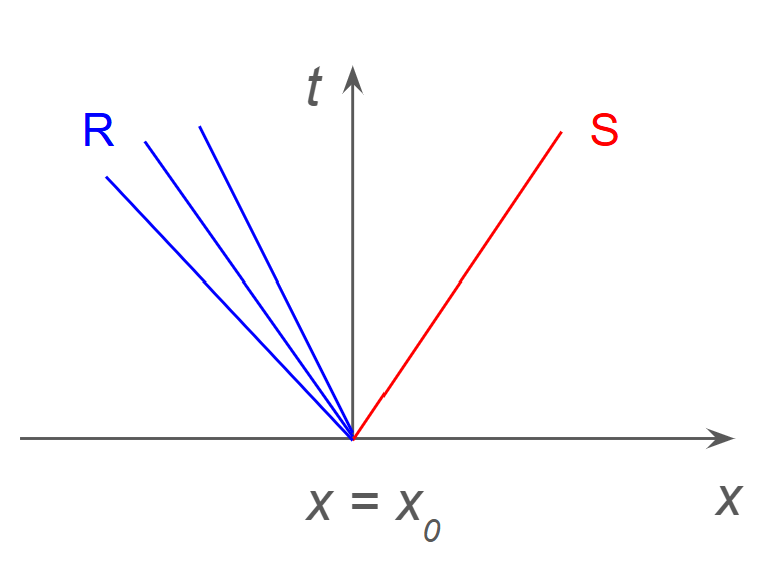
\includegraphics[width=\textwidth]{C:/Users/Matteo/Shallow-Water-Equations/figs/waves-LRRS.png}
        \caption{Left rarefaction wave, right shock wave.}\label{fig:waves-LRRS}
    \end{subfigure}
    \hspace{0.02\textwidth} % Small horizontal space between figures
    \begin{subfigure}[b]{0.4\textwidth}
        \centering
        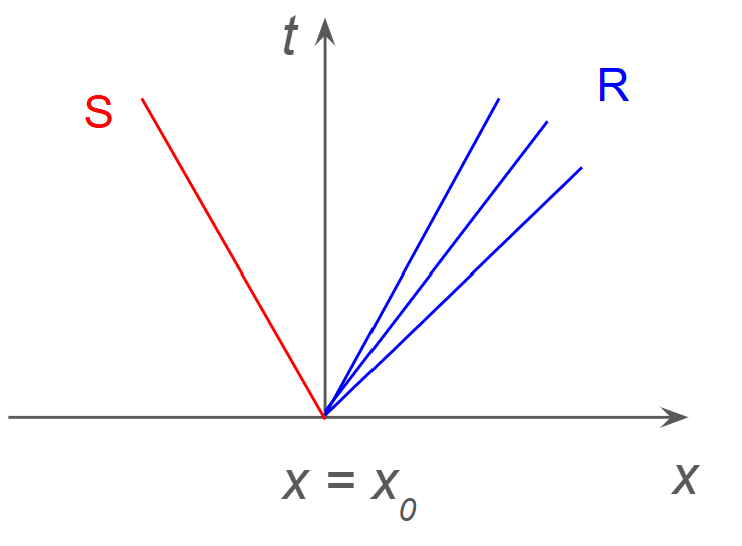
\includegraphics[width=\textwidth]{C:/Users/Matteo/Shallow-Water-Equations/figs/waves-LSRR.png}
        \caption{Left shock wave, right rarefaction wave.}\label{fig:waves-LSRR}
    \end{subfigure}
    
    % Second row
    \begin{subfigure}[b]{0.4\textwidth}
        \centering
        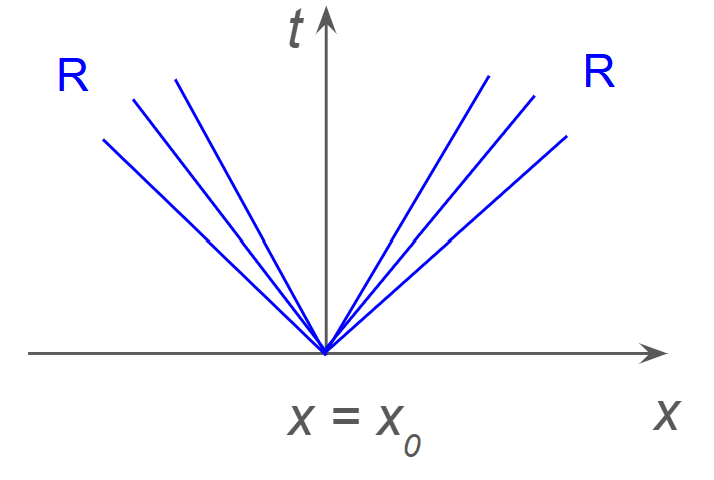
\includegraphics[width=\textwidth]{C:/Users/Matteo/Shallow-Water-Equations/figs/waves-LRRR.png}
        \caption{Left and right rarefaction waves.}\label{fig:waves-LRRR}
    \end{subfigure}
    \hspace{0.02\textwidth} % Small horizontal space between figures
    \begin{subfigure}[b]{0.4\textwidth}
        \centering
        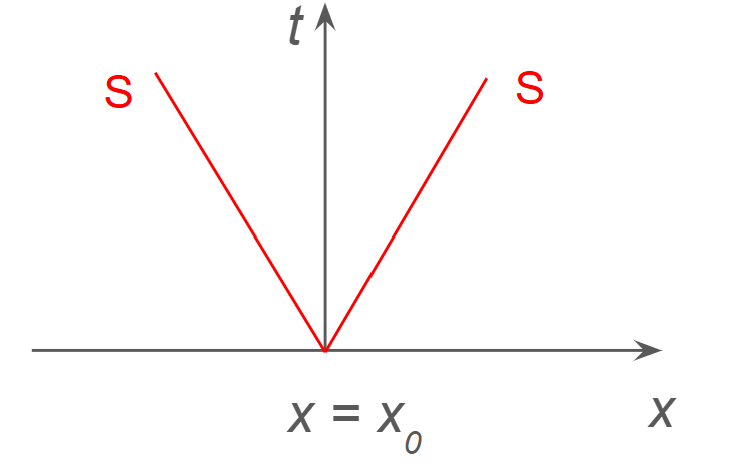
\includegraphics[width=\textwidth]{C:/Users/Matteo/Shallow-Water-Equations/figs/waves-LSRS.png}
        \caption{Left and right shock waves.}\label{fig:waves-LSRS}
    \end{subfigure}
    \caption{Four possible wave patterns in the solution of the Riemann problem.}\label{fig:wave-patterns}
\end{figure}


\subsection{Flux-splitting/Upwind}
In the flux splitting we compute $h_*$ and $u_*$ by assuming a two-rarefaction wave structure.
We define 
\begin{align*}
    c_L = \sqrt{g h_L}, \quad c_R = \sqrt{g h_R},
\end{align*}
to obtain
\begin{align*}
    h_{S2} = {\left( \frac{0.75}{\sqrt{g}} \cdot (q_L - q_R) + 0.5 \cdot \left(h_L^{1.5} + h_R^{1.5}\right) \right)}^2, \\
    h_{S} = h_{S2}^{\frac{1}{3}}
\end{align*}
and
\begin{align*}
    u_* = \frac{1}{2} (u_L + u_R) + \frac{1}{3} \sqrt{g} (h_L^{1.5} - h_R^{1.5}).
\end{align*}




\subsection{Roe solver}
Consider the non-linear Riemann problem in~\eqref{eq:Riemann_problem}:
\begin{align*}
    \mathbf{U}_t + \mathbf{F(U)}_x \equiv \mathbf{U}_t + \mathbf{A} \mathbf{U}_x = 0,
\end{align*}
where $\mathbf{A}$ is the Jacobian matrix of $\mathbf{F}$. 
The Roe solver is based on an approximation of the Jacobian matrix $\mathbf{A}$ by a Roe matrix $\tilde{\mathbf{A}}$, which is a constant coefficient matrix, to obtain the linear system
\begin{align*}
    \mathbf{U}_t + \mathbf{\tilde{A}} \mathbf{U}_x = 0.
\end{align*}

This means that the Roe solver solves the approximated Riemann problem
\begin{align*}
    \mathbf{U}_t + \mathbf{\tilde{A}} \mathbf{U}_x &= 0. \\
    \mathbb{U}(x,0) = \begin{cases}
        \mathbf{U}_L, & x < 0, \\
        \mathbf{U}_R, & x > 0.
    \end{cases}
\end{align*}
exact.
That is, the original non-linear conservation laws are replaced by a linearised system with constant coefficients.

The main idea in the Roe solver is to find average values $\tilde{h}, \tilde{a}, \tilde{u}$ and $\tilde{\psi}$ for the depth $h$, the celerity $a$ (??), the velocity component $u$ and the scalar $\psi$.
The method thus use the following Roe averages:
\begin{align}\label{eq:Roe_averages}
    \left\{
\begin{aligned}
    \tilde{h} &= \sqrt{h_L h_R}, \\
    \tilde{u} &= \frac{u_L \sqrt{h_L} + u_R \sqrt{h_R}}{\sqrt{h_L} + \sqrt{h_R}}, \\
    \tilde{a} &= \sqrt{\frac{1}{2}(a_L^2 + a_R^2)}, \\
    \tilde{\psi} &= \frac{\psi_L \sqrt{h_L}  + \psi_R \sqrt{h_R}}{\sqrt{h_L} + \sqrt{h_R}}.
\end{aligned}
\right.
\end{align}
The average eigenvalues (of what?) are
\begin{align*}
    \tilde{\lambda}_1 = \tilde{u} - \tilde{a}, \quad \tilde{\lambda}_2 = \tilde{u}, \quad \tilde{\lambda}_3 = \tilde{u} + \tilde{a}, \\
\end{align*} 
with the correspinding right eigenvectors
\begin{align*}
    \tilde{\mathbf{R}}^{(1)} = \begin{bmatrix}
        1 \\ \tilde{u} - \tilde{a} \\ \tilde{\psi}
    \end{bmatrix}, \quad
    \tilde{\mathbf{R}}^{(2)} = \begin{bmatrix}
        0 \\ 0 \\  1
    \end{bmatrix}, \quad
    \tilde{\mathbf{R}}^{(3)} = \begin{bmatrix}
        1 \\ \tilde{u} + \tilde{a} \\ \tilde{\psi}
    \end{bmatrix}.
\end{align*}
The wave strenghts $\tilde{\alpha}_j$ described by Roe averages are given by
\begin{align}
    \left\{
    \begin{aligned}
        \tilde{\alpha}_1 &= \frac{1}{2} \left[ \Delta h - \frac{\tilde{h}}{\tilde{a}} \Delta u  \right], \\
        \tilde{\alpha}_2 &= \frac{1}{2} \left[ \tilde{h} \Delta \psi  \right], \\
        \tilde{\alpha}_3 &= \frac{1}{2} \left[ \Delta h + \frac{\tilde{h}}{\tilde{a}} \Delta u  \right].
    \end{aligned}    
    \right.
\end{align}
Applying theory of linear systems with constant coefficients.
The numerical flux is
\begin{align}\label{eq:Roe_flux}
    \mathbf{F}_{i+\frac{1}{2}} = \frac{1}{2} \left( \mathbf{F}_L + \mathbf{F}_R \right) - \frac{1}{2} \sum_{j=1}^3 \tilde{\alpha}_j \left| \tilde{\lambda}_j \right| \tilde{\mathbf{R}}^{(j)}.
\end{align}
The Roe flux~\eqref{eq:Roe_flux} is used in the explicit conservative scheme to solve the SWE in 1D.

Godunov:
Consider the initial-boundary value problem (IBVP) for a system of $N$ nonlinear hyperbolic conservation (balance?) laws     
\begin{equation}\label{eq:IBVP_system}
    \begin{cases}
    \text{PDEs: }    &\mathbf{U}_t + \mathbf{F(U)}_x = \mathbf{S(U)}, \quad x \in [a, b], \quad t > 0, \\
    \text{ICs: }    &\mathbf{U}(x,0) = \mathbf{U}^{(0)}(x), \quad x \in [a,b], \\
    \text{BCs: }    &\mathbf{U}(a,t) = \mathbf{B}_{L}(t), \quad \mathbf{U}(b,t) = \mathbf{B}_{R}(t), \quad t \geq 0.
    \end{cases}
\end{equation}
The vectors $\mathbf{B}_L (t)$ and $\mathbf{B}_R (t)$ denote the boundary conditions at the left and right boundaries, respectively.
The Godunov Upwind method in conservative form~\eqref{eq:explicit_conservative_1D_SWE} solves the IBVP~\eqref{eq:IBVP_system}.
We compute $h_*$ and $u_*$ by starting with a two-rarefaction wave structure, and solve the wetbed problem iteratively.



